\section{Logistische regressie }

\subsection{Classificatie}
Een binaire classificatie zal 2 mogelijke output-waarden hebben die we kunnen voorstellen als een negatieve klasse ($y = 0$) en een positieve klasse ($y = 1$).  We zouden kunnen proberen om een regressie model te fitten op deze data en onze output te voorspellen afhankelijk of de waarde voor $f_{w,b}(x)$ groter of kleiner is dan een drempelwaarde (bijvoorbeeld 0,5). We zullen echter zien dat dit model heel gevoelig is voor uitschieters en dat $f_{w,b}(x)$ groter dan 1 of kleiner dan 0 kan zijn. Dit is ongewenst.\\
\newline
We zouden willen dat $f_{w,b}(x)$ tussen 0 en 1 ligt. Om dit te bereiken kunnen we logistische regressie gebruiken. De naam is een beetje verwarrend maar dit is een geval van classificatie en geen regressie. In de praktijk wordt dit gerealiseerd met een neuraal netwerk met één node. 

\subsection{Logistische regressie }
\label{ch:logistic-regression}
Om ervoor te zorgen dat $f_{w,b}(x)$ tussen 0 en 1 ligt, passen we er de sigmoid of logistische functie op toe. Dit levert ons de volgende vergelijking op: 

\begin{equation}
	f_{\vec{w},b}(\vec{x}) = g(\vec{w} \cdot \vec{x} + b)
	\label{eq:f-wb-log}
\end{equation}
waarbij de sigmoid functie $g(z)$ gelijk is aan:
\begin{equation}
	g(z) = \frac{1}{1 + e^{-z}}
	\label{eq:sigmoid}
\end{equation}
\noindent
We kunnen in deze formule duidelijk zien dat $g(z)$ gelijk zal zijn aan 0 voor kleine waarden voor $z$, dat deze 1 zal zijn voor grote waarden voor $z$ en dat deze gelijk zal zijn aan $\frac{1}{2}$ voor een $z$ die 0 is. Dit wordt ook grafisch weergegeven op Figuur \ref{fig:sigmoid}.

\begin{figure}[h]
	\centering
	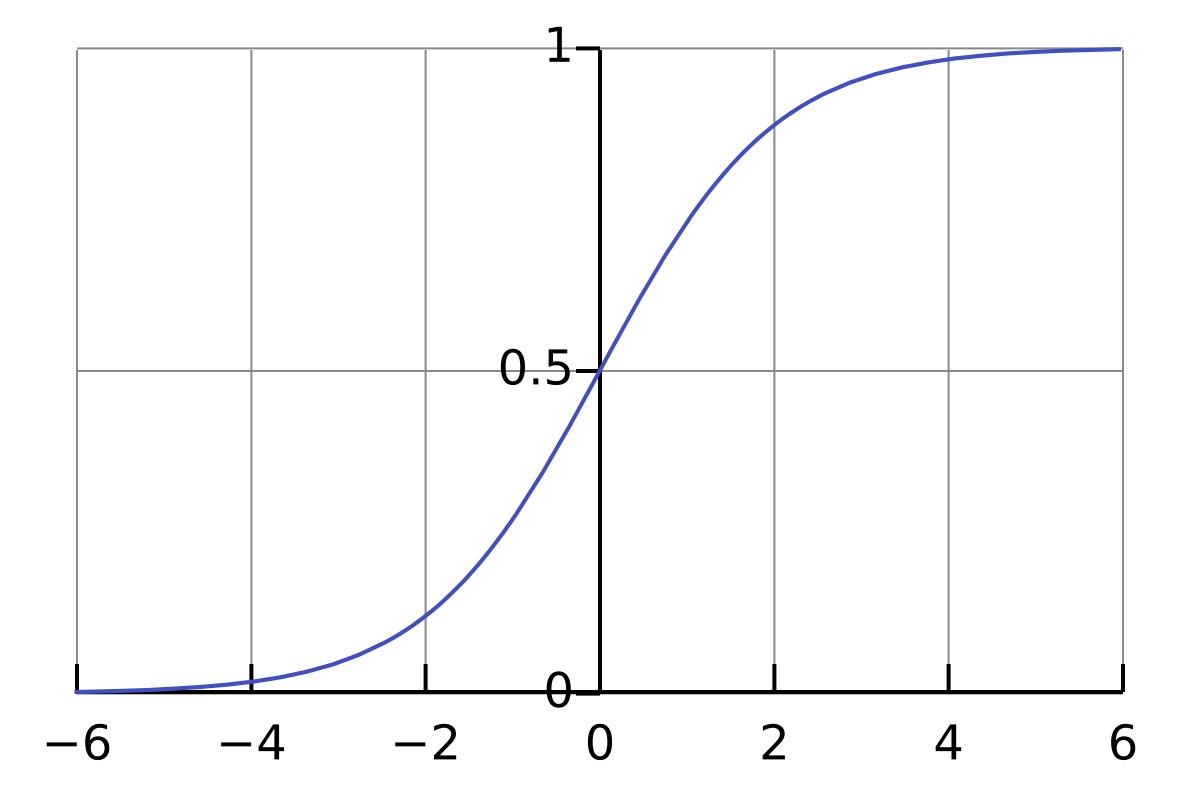
\includegraphics[width=0.45\textwidth]{images/9-sigmoid-function.png}
	\caption{Sigmoid functie $g(z)$}
	\label{fig:sigmoid}
\end{figure}
\newpage
\noindent
Het resultaat van $f_{\vec{w},b}(\vec{x})$ is gelijk aan de kans dat onze $y$ gelijk is aan 1 voor de input $x$. Hiermee kunnen we ook complementen gaan berekenen. 

\paragraph{Sigmoid in Python}

We kunnen de sigmoid functie ook in Python berekenen. Dit ziet er als volgt uit:
\begin{lstlisting}
	def sigmoid(z):
	    """
	    Compute the sigmoid of z
	    Args:
	        z (ndarray): A scalar, numpy array of any size.
	    Returns:
	        g (ndarray): sigmoid(z), with the same shape as z
	    """
	
	    g = 1 / (1 + numpy.exp(-z))
	
	    return g
\end{lstlisting}
\subsection{\textit{Decision boundary}}

We kunnen bijvoorbeeld stellen dat we de waarde 1 toekennen aan onze output als $f_{\vec{w},b}(\vec{x}) \geq 0,5$ of als $z \geq 0$. We kennen dan een waarde 0 toe aan de output als $f_{\vec{w},b}(\vec{x}) < 0,5$ of als $z < 0$. We willen dus dat we zo ver mogelijk van deze waarde 0,5 vandaan zitten omdat we dan zeker zijn van onze output. Deze zone rond 0,5 (rond $z = 0$) noemen we de \textit{decision boundary} (ook wel scheidingsvlak). Dit zal de grens tussen beide klassen zijn. We kunnen dus op basis van de waarde van $z$ ($z < 0, z > 0$ of $z = 0$) bepalen tot welke klasse onze output behoort. Zoals we zien in formule \ref{eq:f-wb-log}, berekenen we $z$ als volgt:

\begin{equation}
	z = \vec{w} \cdot \vec{x} + b = \vec{w}^{T}\vec{x} + b = w_{1}x_{1} + w_{2}x_{2} + \ldots + w_{n}x_{n} + b
\end{equation}

\subsection{Kostfunctie voor logistische regressie}

De kostfunctie zoals we die eerder gezien hebben (formule \ref{eq:cost-function-multi}), zal niet werken voor $f_{\vec{w},b}(\vec{x}) = \frac{1}{1 + e^{-(\vec{w} \cdot \vec{x} + b)}}$. In tegenstelling tot bij lineaire regressie, zal deze bij logistische regressie namelijk niet convex zijn. Bij logistische regressie ziet de \textit{loss}-functie er als volgt uit:

 \begin{equation}
 	L(f_{\vec{w},b}(\vec{x}^{(i)}), y^{(i)}) = \left\{ \begin{matrix} -\ln(f_{\vec{w},b}(\vec{x}^{(i)})) & \mbox{voor } y^{(i)} = 1 \\ -\ln(1 - f_{\vec{w},b}(\vec{x}^{(i)}))  & \mbox{voor } y^{(i)} = 0 \end{matrix}\right .
 	\label{eq:loss-function-log}
 \end{equation}
\noindent
Wanneer we deze verliesfuncties plotten voor $y^{(i)} = 1$ en $y^{(i)} = 0$, zien we dat het de \textit{loss} het laagste is wanneer $f_{\vec{w},b}(\vec{x}^{(i)})$ dicht aansluit bij zijn werkelijk label $y^{(i)}$ (Figuur \ref{fig:loss-function-log}). Op de horizontale as zien we $f_{\vec{w},b}(\vec{x}^{(i)})$ en op de verticale as zien we $L(f_{\vec{w},b}(\vec{x}^{(i)}), y^{(i)})$.

\begin{figure}[h]
	\centering
	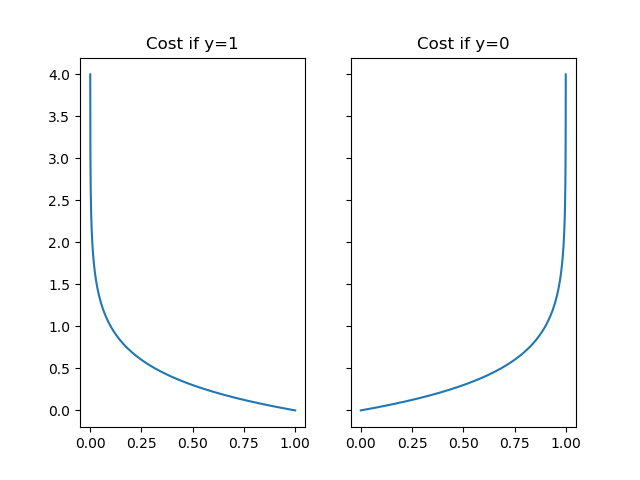
\includegraphics[width=0.5\textwidth]{images/10-loss-function-log.png}
	\caption{Verliesfunctie voor logistische regressie}
	\label{fig:loss-function-log}
\end{figure}
\noindent
We krijgen vervolgens een kostfunctie die er als volgt uit ziet:
\begin{equation}
	J(\vec{w}, b) = \frac{1}{m} \sum_{i=1}^{m} L(f_{\vec{w},b}(\vec{x}^{(i)}), y^{(i)})
	\label{eq:cost-function-log}
\end{equation}
\noindent
Wanneer we formule \ref{eq:loss-function-log} en formule \ref{eq:cost-function-log} combineren, bekomen we de volgende vereenvoudigde kostfunctie:
\begin{equation}
	J(\vec{w}, b) = -\frac{1}{m} \sum_{i=1}^{m} y^{(i)}\ln(f_{\vec{w},b}(\vec{x}^{(i)})) + (1 - y^{(i)}) \ln(1 - f_{\vec{w},b}(\vec{x}^{(i)})) 
	\label{eq:cost-function-log-simp}
\end{equation}
\noindent
Wanneer het label $y^{(i)}$ gelijk is aan 1, zal enkel de eerste term uit formule \ref{eq:cost-function-log-simp} meetellen aangezien $(1 - y^{(i)})$ dan gelijk is aan 0. Wanneer het label $y^{(i)}$ gelijk is aan 0, zal op gelijkaardige manier enkel de tweede term uit formule \ref{eq:cost-function-log-simp} meetellen. Deze kostfunctie zal wel een convex verloop hebben. In de literatuur wordt er ook wel eens gesproken over \textit{logistic loss} of \textit{crossentropy loss}.

\paragraph{De kostfunctie in Python}
In Python kunnen we de kostfunctie als volgt berekenen:
\begin{lstlisting}
	def compute_cost(X, y, w, b):
	    """
	    Computes the cost over all examples
	    Args:
	        X : (ndarray Shape (m,n)) data, m examples by n features
	        y : (array_like Shape (m,)) target value 
	        w : (array_like Shape (n,)) Values of parameters of the model      
	        b : scalar Values of bias parameter of the model
	    Returns:
	        total_cost: (scalar)         cost 
	    """
	
	    m, n = X.shape
	
	    loss_sum = 0 
\end{lstlisting}
\newpage
\begin{lstlisting}	
	    # Loop over each training example
	    for i in range(m): 
	
	        # First calculate z_wb = w[0]*X[i][0]+...+w[n-1]*X[i][n-1]+b
	        z_wb = numpy.dot(w, X[i]) + b
	
	        # Calculate prediction f_wb for a training example
	        f_wb = sigmoid(z_wb)
	        # Calculate loss for a training example
	        loss =  (-y[i]*numpy.log(f_wb))-(1-y[i])*numpy.log(1-f_wb)
	        # Add the loss to the total loss
	        loss_sum += loss
	
	    total_cost = (1 / m) * loss_sum  
	
	    return total_cost
\end{lstlisting}

\subsection{\textit{Gradient descent} voor logistische regressie}

We willen opnieuw de kostfunctie minimaliseren en dit kan opnieuw met \textit{gradient descent}. Dit gebeurt op dezelfde manier als bij lineaire regressie (formule \ref{eq:gradient-descent-lin-reg-multi-w} en formule \ref{eq:gradient-descent-lin-reg-multi-b}), al zal $f_{\vec{w},b}(\vec{x})$ hier natuurlijk wel gelijk zijn aan $g(\vec{w} \cdot \vec{x} + b)$ in plaats van $\vec{w} \cdot \vec{x} + b$.

\paragraph{\textit{Gradient descent} in Python}

We kunnen opnieuw \textit{gradient descent} uitrekenen in Python. De volgende functie laat ons toe om de gradiënt te berekenen:
\begin{lstlisting}
	def compute_gradient(X, y, w, b, lambda): 
	    """
	    Computes the gradient for logistic regression 
	    Args:
	        X : (ndarray Shape (m,n)) variable such as house size 
	        y : (array_like Shape (m,1)) actual value 
	        w : (array_like Shape (n,1)) values of parameters of the model      
	        b : (scalar) Value of parameter of the model 
	    Returns
	        dj_dw: (array_like Shape (n,1)) The gradient of the cost w.r.t. the parameters w. 
	        dj_db: (scalar)                The gradient of the cost w.r.t. the parameter b. 
	    """
	    m, n = X.shape
	    dj_dw = numpy.zeros(w.shape)
	    dj_db = 0.
	
	    for i in range(m):
	        # Calculate f_wb
	        f_wb = sigmoid(numpy.dot(w,X[i])+b)
	
	        # Calculate the  gradient for b from this example
	        dj_db_i = f_wb - y[i]
	
	        # Add that to dj_db
	        dj_db += dj_db_i
\end{lstlisting}
\newpage
\begin{lstlisting}	
	        # Get dj_dw for each attribute
	        for j in range(n):
	            # Calculate the gradient from the i-th example for j-th attribute
	            dj_dw_ij = (f_wb - y[i]) * X[i,j]
	            dj_dw[j] += dj_dw_ij
	
	    # divide dj_db and dj_dw by total number of examples
	    dj_dw = dj_dw / m
	    dj_db = dj_db / m
	
	    return dj_db, dj_dw
\end{lstlisting}
\noindent
\\
We kunnen deze functie opnieuw gebruiken om de waarden van onze parameters aan te passen zoals in formule \ref{eq:gradient-descent-lin-reg-multi-w} en formule \ref{eq:gradient-descent-lin-reg-multi-b}:
\begin{lstlisting}
	"""
	X : (array_like Shape (m, n)
	y : (array_like Shape (m,))
	w_in : (array_like Shape (n,)) Initial values of parameters of the model
	b_in : (scalar) Initial value of parameter of the model
	alpha : (float) Learning rate
	num_iters : (int) Number of iterations to run gradient descent
	"""
	for i in range(num_iters):
	    # Calculate the gradient and update the parameters
	    dj_db, dj_dw = compute_gradient(X, y, w_in, b_in)   
	
	    # Update Parameters using w, b, alpha and gradient
	    w_in = w_in - alpha * dj_dw               
	    b_in = b_in - alpha * dj_db 
\end{lstlisting}

\paragraph{Predictie in Python}

We kunnen vervolgens ook een functie opstellen die een voorspelling maakt over ons label op basis van de geleerde parameters $w$ en $b$:

\begin{lstlisting}
	def predict(X, w, b): 
	    """
	    Predict whether the label is 0 or 1 using learned logistic regression parameters w and b
	    Args:
	        X : (ndarray Shape (m, n))
	        w : (array_like Shape (n,)) Parameters of the model
	        b : (scalar, float) Parameter of the model
	    Returns:
	        p: (ndarray (m,1)) The predictions for X using a threshold at 0.5
	    """
	    # number of training examples
	    m, n = X.shape   
	    p = numpy.zeros(m)
	
	    # Loop over each example
	    for i in range(m):   
	        # Calculate f_wb 
	        f_wb = sigmoid(numpy.dot(w,X[i])+b)
\end{lstlisting}
\newpage
\begin{lstlisting}		
	        # Calculate the prediction for that training example 
	        p[i] = 1 if (f_wb >= 0.5) else 0
	
	    return p
\end{lstlisting}

\subsection{Regularisatie}
\subsubsection{\textit{Under- en overfitting}}
Wanneer onze kostfunctie heel laag of zelfs 0 is, hebben we een model dat heel goed aansluit bij onze trainingsdata. Het zal echter niet goed aansluiten bij nieuwe data en is dus te complex om er aan te voldoen. We spreken dan van \textit{overfitting} of \textit{high variance}. Dit is zichtbaar op de linkergrafiek van Figuur \ref{fig:overfitting-underfitting}. \\
\newline
Wanneer onze kostfunctie hoog is, hebben we een model dat niet goed aansluit bij onze data en te simpel is om er aan te voldoen. We spreken dan van \textit{underfitting} of \textit{high bias}. Dit is zichtbaar op de rechtergrafiek van Figuur \ref{fig:overfitting-underfitting}. \\
\newline
Idealiter bevinden we ons dus in een situatie zoals de middelste grafiek van Figuur \ref{fig:overfitting-underfitting}. Hier zullen we een fit hebben die redelijk goed aansluit bij onze data en een kostfunctie die groter is dan bij \textit{overfitting}, maar kleiner dan bij \textit{underfitting}. De \textit{decision boundary} zal dan ook tussen die van de andere gevallen in liggen.

\begin{figure}[h]
	\centering
	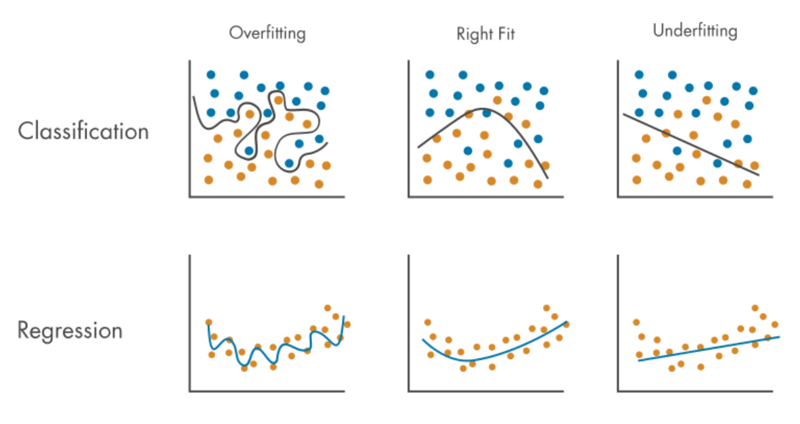
\includegraphics[width=\textwidth]{images/11-overfitting-underfitting.png}
	\caption{\textit{Overfitting}, \textit{underfitting} en een goeie fit}
	\label{fig:overfitting-underfitting}
\end{figure}

\subsubsection{\textit{Overfitting} tegengaan}

Er zijn een aantal opties die we kunnen toepassen om \textit{overfitting} tegen te gaan:
\begin{itemize}
	\item Het aantal \textit{features} reduceren (\textit{feature selection / reduction}). Dit gebeurt vooral op basis van domeinkennis.
	\item Meer trainingsdata toevoegen
	\item Regularisatie
\end{itemize}

\subsubsection{Regularisatie}

Bij regularisatie willen we het aandeel van bepaalde \textit{features} afstraffen zodat ze een minder grote invloed hebben om zo \textit{overfitting} tegen te gaan. Dit kunnen we doen door de overeenkomstige gewichten te betrekken in de kostfunctie, zodat deze ook geminimaliseerd zullen worden. 

\paragraph{Regularisatie bij lineaire regressie}

Voor lineaire regressie bekomen we dan de volgende kostfunctie wanneer we regularisatie toepassen:

\begin{equation}
	J(\vec{w}, b) = \frac{1}{2m} \sum_{i=1}^{m} (f_{\vec{w},b}(\vec{x}^{(i)}) - y^{(i)})^{2} + \frac{\lambda}{2m} \sum_{j=1}^{n} w_{j}^{2}
	\label{eq:cost-function-lin-regul}
\end{equation}
\noindent
Deze kostfunctie bestaat nu uit twee termen die elk hun eigen doel hebben. De eerste term heeft als doel om de data te fitten. De tweede term zal \textit{overfitting} trachten te compenseren. Hier is $\lambda$ een hyperparameter die ook wel de regularisatieparameter genoemd wordt. Wanneer deze te hoog wordt ingesteld, lopen we het risico op \textit{underfitting} aangezien de gewichten dan allemaal heel klein zullen zijn en vooral de constante \textit{bias} een invloed zal hebben. \\
\newline
In onze formules voor het \textit{gradient descent} algoritme, zal dit leiden tot een extra term $-\frac{\alpha \lambda}{m} w_{j}$ in formule \ref{eq:gradient-descent-lin-reg-multi-w}. Formule \ref{eq:gradient-descent-lin-reg-multi-b} zal ongewijzigd blijven aangezien deze term wegvalt wanneer we J($\vec{w}$, b) afleiden naar $b$. We kunnen hier dus ook weer terugzien dat de regularisatie ervoor zorgt dat de invloed van het gewicht afneemt. In de literatuur spreken we van \textit{weight decay}. 

\paragraph{Regularisatie bij logistische regressie}

Op dezelfde manier als in formule \ref{eq:cost-function-lin-regul}, zal er na toepassing van regularisatie een extra term toegevoegd worden aan de kostfunctie:
\begin{equation}
	J(\vec{w}, b) = -\frac{1}{m} \sum_{i=1}^{m} y^{(i)}\ln(f_{\vec{w},b}(\vec{x}^{(i)})) + (1 - y^{(i)}) \ln(1 - f_{\vec{w},b}(\vec{x}^{(i)})) + \frac{\lambda}{2m} \sum_{j=1}^{n} w_{j}^{2}
\end{equation}
\noindent
Deze kostfunctie bestaat opnieuw uit twee termen die elk dezelfde doelen hebben als hierboven. Dit zal opnieuw leiden tot dezelfde extra term voor de \textit{weight decay} bij het toepassingen van \textit{gradient descent}.

\paragraph{Regularisatie in Python}

We kunnen de formules om de kostfunctie te berekenen en om \textit{gradient descent} toe te passen uitbreiden in Python om regularisatie toe te voegen. Dit levert ons de volgende Python-code op:

\begin{lstlisting}
	def compute_cost_reg(X, y, w, b, lambda_ = 1):
	    """
	    Computes the cost over all examples
	    Args:
	        X : (array_like Shape (m,n)) data, m examples by n features
	        y : (array_like Shape (m,)) target value 
	        w : (array_like Shape (n,)) Values of parameters of the model      
	        b : (array_like Shape (n,)) Values of bias parameter of the model
	        lambda_ : (scalar, float)    Controls amount of regularization
	    Returns:
	        total_cost: (scalar)         cost 
	    """
	
	    m, n = X.shape
	
	    # Calls the compute_cost function that we implemented before
	    cost_without_reg = compute_cost(X, y, w, b) 
\end{lstlisting}
\begin{lstlisting}
	    # We need to calculate this value
	    reg_cost = 0.
	
	    for j in range(n):
	        reg_cost_j = w[j]**2
	        reg_cost = reg_cost + reg_cost_j
	
	    # Add the regularization cost to get the total cost
	    total_cost = cost_without_reg + (lambda_/(2 * m)) * reg_cost
	
	    return total_cost
\end{lstlisting}
\begin{lstlisting}	
	def compute_gradient_reg(X, y, w, b, lambda_ = 1): 
	    """
	    Computes the gradient for linear regression 
	    Args:
	        X : (ndarray Shape (m,n))   variable such as house size 
	        y : (ndarray Shape (m,))    actual value 
	        w : (ndarray Shape (n,))    values of parameters of the model      
	        b : (scalar)                value of parameter of the model  
	        lambda_ : (scalar,float)    regularization constant
	    Returns
	        dj_db: (scalar)             The gradient of the cost w.r.t. the parameter b. 
	        dj_dw: (ndarray Shape (n,)) The gradient of the cost w.r.t. the parameters w. 
	    """
	    m, n = X.shape
	
	    dj_db, dj_dw = compute_gradient(X, y, w, b)
	
	    # Loop over the elements of w
	    for j in range(n): 
	        # Calculate the regularization term for dj_dw[j]
	        dj_dw_j_reg = (lambda_ / m) * w[j]
	
	        # Add the regularization term  to the correspoding element of dj_dw
	        dj_dw[j] = dj_dw[j] + dj_dw_j_reg
	
	    return dj_db, dj_dw
\end{lstlisting}
